\section{Gradient-Based Methods}
This section provides a theoretical introduction to gradient based methods. First, \ref{itm:attribution}-approaches (\cref{subsect:lrp,subsect:td,subsect:dtd}) are presented, then \ref{itm:signal}-approaches \cref{subsect:guided-backprop}. Finally, \cref{subsect:patternnet-attribution} are discussed, where PatternNet is a \ref{itm:signal}-approach and PatternAttribution a \ref{itm:attribution}-approach.

\subsection{Layer-Wise Relevance Decomposition}
\blindtext[3]

\subsubsection{Taylor-Decomposition}
\blindtext[3]

\subsubsection{Deep-Taylor-Decomposition}
\blindtext[3]
\subsection{Taylor-Decomposition}\label{subsect:td}
As an approximation to \gls{lrp}, \gls{td} was proposed in~\cite{Bach.2015}. It directly defines relevances \(R_{h}^{(1)}\) at the (slightly modified) input-sample \(x'\) and therefore avoids the process of decomposing relevances for each layer. Instead, relevance \(R_{h}^{(1)}\) is defined by developing a first order Taylor series of the input \(x\) around a root point \(x_0\), such that \(f(x_0) = 0\). Informally, \gls{td} attributes relevance by weighting the difference of the image and the root point (\(x-x_0\)) with the partial derivative of the model with respect to the input \(x\). Formally
\begin{equation}
    R_{h}^{(1)} \approx (x-x_0)_{(h)} * \frac{\partial f}{\partial x_{(h)}}(x_0).
\end{equation}
Here, \(x'\) as mentioned above is \(x':=x-x_0\).
\par
Again, a set of constraints is formulated to find the root-point \(x_0\)
\begin{enumerate}
    \item \(x_0\) must be a root point of \(f\), such that \(f(x_0)=0\)
    \item \(x_0\) must be in the neighborhood of \(x\) under some distance metric, e.g.\ the Euclidean L2-norm.\label[const]{enum:taylor-closeness}
\end{enumerate}
A major issue with \gls{td} is satisfying \cref{enum:taylor-closeness}. \fcite{Bach.2015} do not provide a solution for sparsely populated data-domains, e.g.\ datasets of natural images. Yet, when the root point is ill-defined, \fcite{Kindermans.2019} were able to show that \gls{td} produces bad results.
\subsection{Deep-Taylor-Decomposition}\label{subsect:dtd}
\gls{dtd} as proposed by \fcite{Montavon.2017} tries to overcome the difficulties that the search for root-points according to \cref{enum:taylor-closeness} posed to simple \gls{td}. For this, they introduce axioms \ref{ax:positivity} and \ref{ax:consistency} which \gls{dtd} must satisfy. Also, they propose a method for finding root-points \(x_0(i):= x_i + t*v_i\), where \(v_i\) is called \textit{search direction}. \citeauthor{Montavon.2017} use this definition to define a set of weighting terms, similar to those in \gls{lrp} and \gls{td}. Formally, they introduce a generalization of the weighting parameter in \cref{eq:weighting-in-dtd}\cite[see][Supplementary Material]{Montavon.2017}
\begin{equation}
    R_{i\leftarrow j}^{(l,l+1)} = \sum_j \frac{v_i w_{ij}}{\sum_i v_i w_{ij}} R_j^{(l+1)}\label{eq:weighting-in-dtd}
\end{equation}
and then derive specific weighting parameters by defining \(v_i\).
\begin{description}
    \item[\namedlabel{itm:w2weighting}{\(\symbfit{w^2}\)-Weighting}{\(\symbfit{w^2}\)-weighting}] which is similar to \cref{eq:weighted-message} but does only rely on the weights \(w_{ij}\) that connect \(i \text{ and } j\). \(v_i\) is chosen to be \(v_i:=w_{ij}\).
    \begin{equation}
        R_{i\leftarrow j}^{(l,l+1)} = R_{j}^{(l+1)} \frac{w_{ij}^2}{\sum_{h\in (l)} w_{hj}^2}.\label{eq:w2-weighting-dtd}
    \end{equation}
    \(w^2\)-weighting is used, when the input-domain is unrestricted, i.e.\ \(x\in \mathbb R^{|x|}\).
    \item[\namedlabel{itm:z+weighting}{\(\symbfit{z^+}\)-Weighting}{\(\symbfit{z^+}\)-weighting}] is equal to the \(\alpha\beta\)-Rule of \gls{lrp}, with \(\beta=0, \alpha=1\). Here, \(v_i\) is the set of all \(x_i\) for which the correspoding \(w_{ij}\) is positive, formally \(w_{ij}^{+} = \left\{w_{ij} | w_{ij}\geq 0\right\}\) and \(v_i:=\left\{x_i|w_{ij}\in w_{ij}^{+}\right\}\). The weighting therefore is
    \begin{equation}
        R_{i\leftarrow j}^{(l,l+1)} = R_{j}^{(l+1)} \frac{x_i w_{ij}^{+}}{\sum_{h\in (l)} x_(h) w_{hj}^{+}}.\label{eq:dtd-z+}
    \end{equation}
    In~\cite{Montavon.2017}, \cref{eq:dtd-z+} is modeled with \(x_i w_{ij}^{+}=:z_{ij}^{+}\), from which the name \(z^{+}\)-weighting is derived.
    \(z^{+}\)-weighting is used, when the input-domain is restricted to positive values, for example in a setting with ReLU-activations, i.e.\ \(x\in \mathbb R_{+}^{|x|}\). A generalization of the \(z^{+}\)-weighting, as discussed in~\cite{Montavon.2017}, is equal to \(\alpha\beta\)-\gls{lrp}.
    \item[\(\symbfit{z^{\mathscr B}}\)-Weighting] is used, when the input-domain is restricted to an upper- and lower-bound, for example in image-classification tasks. For details, please refer to~\cite[215\psq]{Montavon.2017}
\end{description}
\par
In contrast to \gls{td}, \gls{dtd} defines not immediately the relevance at the input-sample \(R_{h}^{(1)}\), but only the relevance of \glspl{message}. It therefore incorporates ideas of both \gls{lrp} (relevance-propagation, even partial equality with the generalization of \ref{itm:z+weighting}) and \gls{td} (approximation of function value with respect to a root-point \(x_0\)). The relevance at the input-sample is recieved by a relevance model that then propagates the \glspl{message} from \(f(x)\) to \(R_{h}^{(1)}\).
\paragraph{Relevance-Models}
\begin{figure*}[ht]
    \center{}
    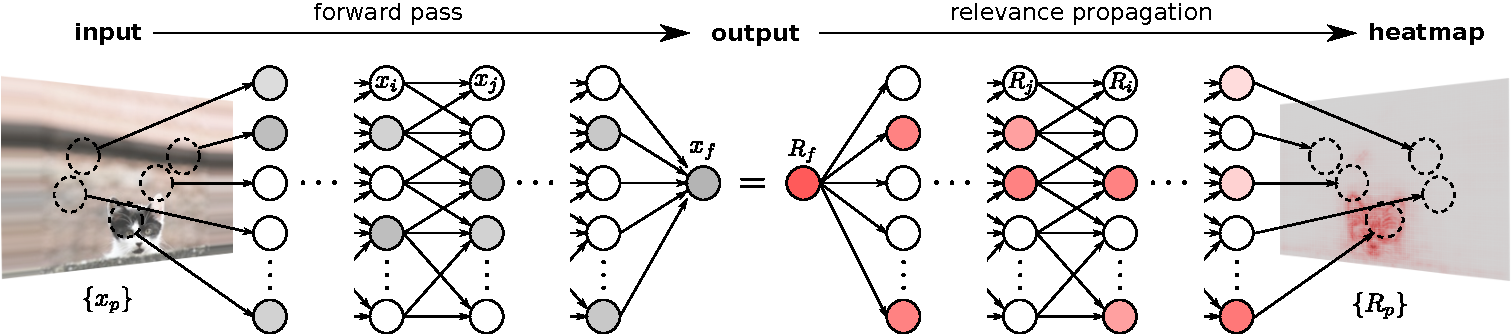
\includegraphics[width=\textwidth]{dtd-flow}
    \caption[Deeper Neural Network; prediction and propagation via \gls{dtd}]{\textbf{Left:} A neural network at prediction time. \textbf{Right:} exemplary \gls{dtd} Relevance Model, adopted from \protect\cite{Montavon.2017}. Note, that in this work, usually \(R_h\) is used instead of \(R_p\).}\label{fig:dtd-nn}
\end{figure*}
\fcite{Montavon.2017} propose two relevance models (\textit{Min-Max Relevance Model} and \textit{Training-free Relevance Model}), for which details are provided in~\cite{Montavon.2017}. They are presented as an inversion of the original \gls{nn}, incorporating their structure. However, no explicit constraints on this property are formulated. The flow in a relevance model is visually depicted in \cref{fig:dtd-nn}. First a prediction \(f(x)=:x_f\) is made (left side) which is then fed through the Relevance Model which extends \(R_f:=x_f\) back to the input sample. While the \textit{Training-free Relevance Model} must, as its name suggests, not be trained, the \textit{Min-Max Relevance Model} has to be trained in a supervised fashion. \fcite{Montavon.2017} show that both, the training-free and min-max relevance models, lead to very similar results.
\subsection{Guided Backprop}
\blindtext[1]
\subsection{PatternNet and PatterAttribution}\label{subsect:patternnet-attribution}
Using either a simple linear model~\cite{Kindermans.2018} or a constant shift in mean~\cite{Kindermans.2019}, \citeauthor{Kindermans.2018} were able to show the vulnerability of gradient methods (such as \gls{lrp}, \gls{td}, \gls{dtd}, Gradient x Input, and Integrated Gradients) to random changes in the input-sample (see \cref{fig:kindermans-unreliability}).
\begin{figure*}
    \center{}
    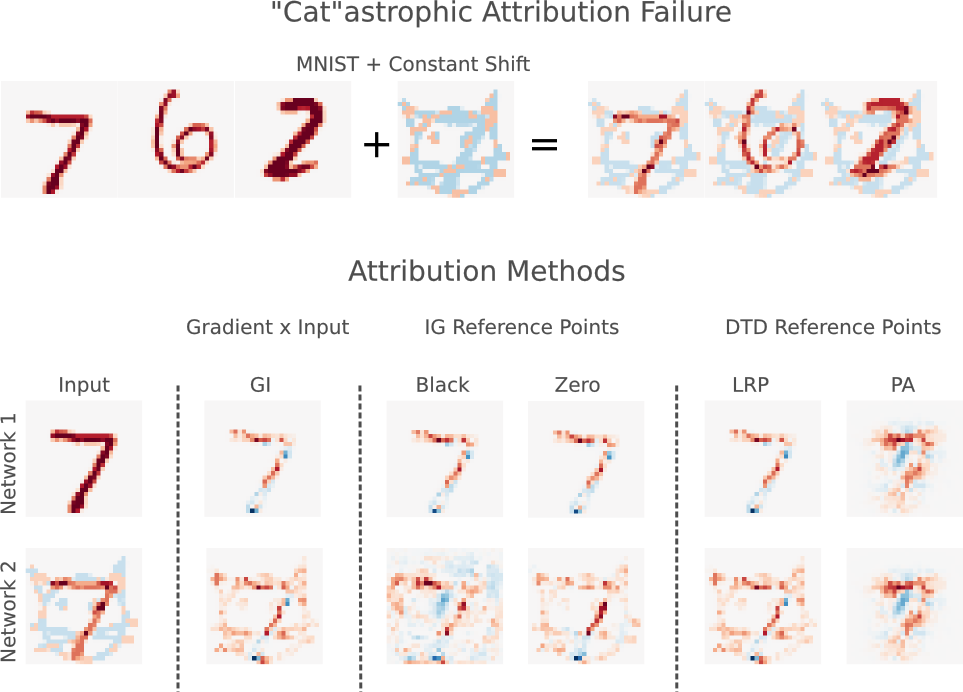
\includegraphics[width=\textwidth]{kindermans-catastrophic-attribution}
    \caption[Evaluation of attribution methods via a constant shift on MNIST]{Evaluation of attribution methods on two models (Network 1 and Network 2). Network 1 is trained on the well known MNIST-Dataset, while Network 2 is trained on a manipulated Version of MNIST with a constant shift (i.e. a hand-drawn image of a cat). Because the constant shift does not add any information to an image, a consistent attribution method should provide a similar explanation for both Network 1 and Network 2, when applied to the same input image with only the constant shift. However, Gradient x Input, Integrated Gradients and \gls{lrp} show a difference between Network 1 and Network 2. For further details, refer to~\cite{Kindermans.2019} from where this figure was adopted.}
    \label{fig:kindermans-unreliability}
\end{figure*}
To overcome this vulnerability of preexisting methods, \fcite{Kindermans.2018} introduce \textit{signal estimators} \(S(x)\) that will be explained in this subsection. Signal estimators root in the idea that each input-sample \(x\) of a dataset is a combination of underlying signal \(s\) (contains all information about e.g.\ the correct class) and distractor \(d\) (does not contain any information about e.g\ the correct class) such that \(x=s\circ d\), with \(\circ\) being some operation, for simplicity let \(\circ\) denote summation \(\circ:=+\)~\cite{Kindermans.2018}. A signal estimator \(S(x)\) is then used to extract \(d\) from \(x\), such that for an optimal signal estimator: \(s = x - S(x)\).
\begin{description}
    \item[\namedlabel{itm:sw-signal-estimator}{The Filter-Based Estimator \(\symbfit{S_w}\)}{\(\symbfit{S_w}\)}] is equal to the \ref{itm:w2weighting} discussed in \cref{subsect:dtd}.
    \begin{equation}
        S_w = \frac{w_{ij}^2}{\sum_{h\in (l)} w_{hj}^2}.
    \end{equation}
    Although simple, \fcite{Kindermans.2018} show that \(S_w(x)\) neither holds theoretically, being unable to separate \(s\) and \(d\), nor empirically as shown in \cref{fig:kindermans-signal-estimator-comparison}.
    \item[\namedlabel{itm:sa-signal-estimator}{The Linear Estimator {}\(\symbfit{S_a}\)}{\(\symbfit{S_a}\)}] is based on the assumption of a linear perceptron. Although this assumptions does not even hold for simple ReLU's, it provides a significant improvement over \ref{itm:sw-signal-estimator} as shown in \cref{fig:kindermans-signal-estimator-comparison}.
    \begin{equation}
        S_{a(i)}(x) = x_{(i)} (a_{(i)} w_{ij})\label{eq:linear-estimator}
    \end{equation}
    please note that, while the weights \(w_{ij}\), which are taken from a trained model, and the input-variable of the input-sample \(x_{(i)}\) are fixed parameters, \(a_{(i)}\) must be trained on a given dataset. Details on the training are provided in~\cite{Kindermans.2018}. \Cref{eq:linear-estimator} is an exemplary formulation of \(S_a\) for the input layer.
    \item[\namedlabel{itm:sa+-signal-estimator}{The Two-Component Estimator \(\symbfit{S_{a+-}}\)}{\(\symbfit{S_{a+-}}\)}] is tailored to ReLU-activation functions. \fcite{Kindermans.2018} notice that due to applying ReLU's, the weights used in previous signal estimators \ref{itm:sw-signal-estimator}, \ref{itm:sa-signal-estimator} are only trained on positive signal \(s_{+}\) and distractor \(d_{+}\) values. To account also for negative \(s_{-}, d_{-}\), they split the estimator accordingly
    \begin{equation}
        S_{a+-(i)} = 
        \begin{cases}
            x_{(i)} (a_{+(i)} w_{ij}),& {\scriptstyle \text{if } (x_{(i)} w_{ij}) > 0}\\
            x_{(i)} (a_{-(i)} w_{ij}),& {\scriptstyle \text{otherwise}}
        \end{cases}
    \end{equation}
    again note that, while the weights \(w_{ij}\) and the input-variable \(x_{(i)}\) are fixed parameters, \(a_{+(i)}, a_{-(i)}\) must be trained on a given dataset. Details on the training are provided in~\cite{Kindermans.2018}.
\end{description}\label{desc:signal-estimators}
\par
In summary, \citeauthor{Kindermans.2018} propose 
\begin{enumerate*}[label={\roman*)}]
    \item the concept of signal estimators in order to overcome the vulnerability of previous methods to a constant-shift in the input and
    \item two new signal estimators, \ref{itm:sa-signal-estimator} and \ref{itm:sa+-signal-estimator}, which significantly improve upon the previously (and naively) used estimator \ref{itm:sw-signal-estimator}.
\end{enumerate*} A visual example for the three signal estimators is provided in \cref{fig:kindermans-signal-estimator-visually}.
\par
For \textit{PatternAttribution}, \fcite{Kindermans.2018} then use the derived signal estimator as a weighting parameter in the \gls{dtd}-framework, which can be interpreted as an informed choice of root-point \(x_0\).
For \textit{PatternNet}, only the signal itself is reconstructed.% \todo{sHOw aN iMaGE oF THiS}
\begin{figure*}[ht]
    \center{}
    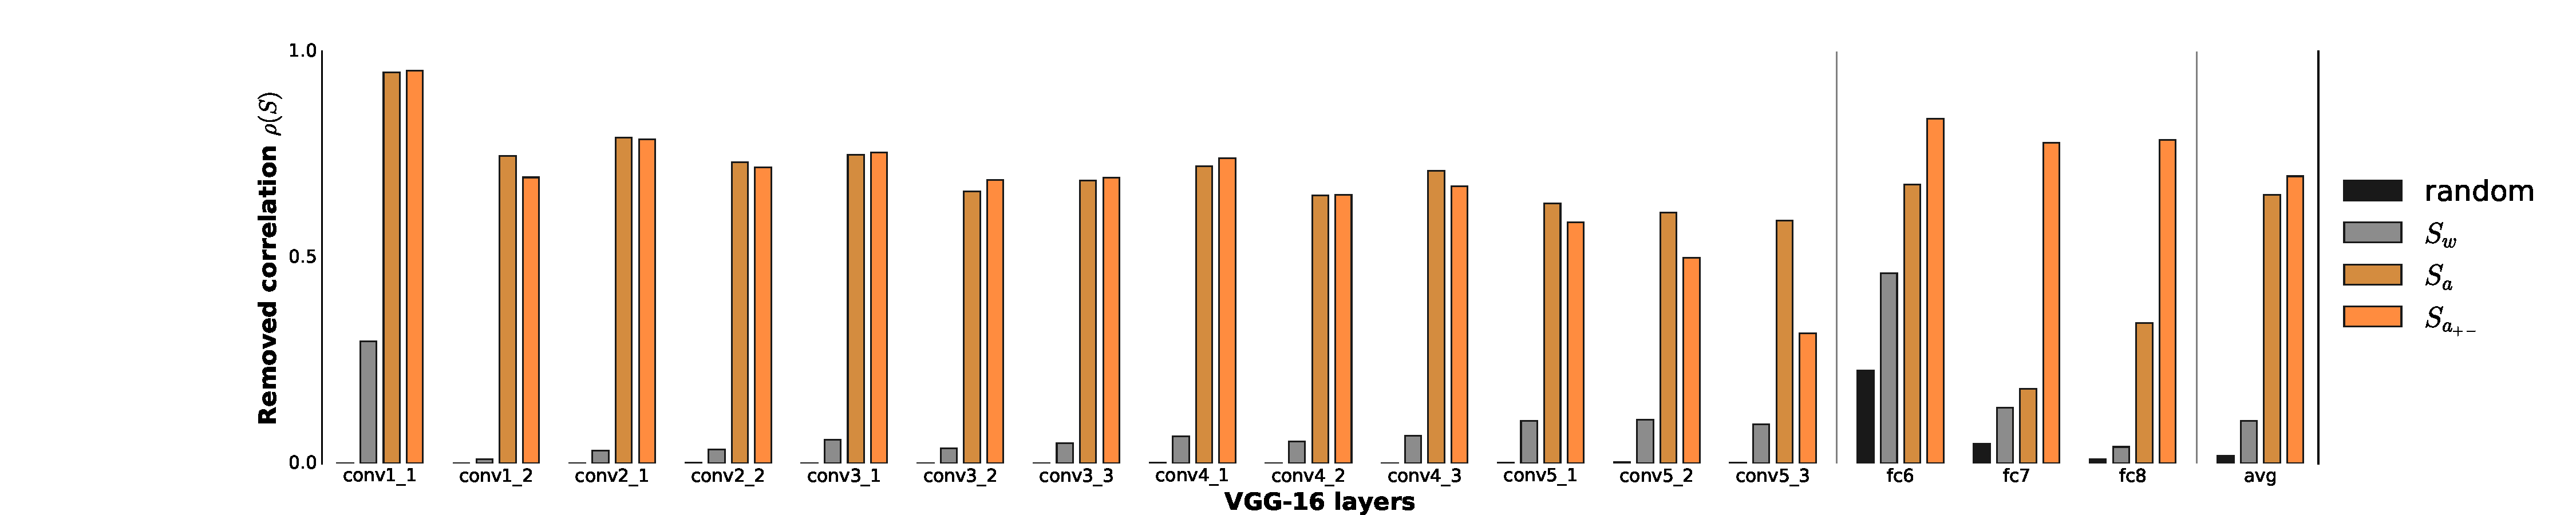
\includegraphics[width=\textwidth]{kindermans-signal-estimators}
    \caption[Evaluation of Signal Estimators for VGG-16 on different layers.]{Evaluation of Signal Estimators for VGG-16 on different layers. Higher values are better. A random Signal Estimator is used as baseline. For details on the quality measure \(\rho\) refer to \cite{Kindermans.2018} from where this figure was adopted.}
    \label{fig:kindermans-signal-estimator-comparison}
\end{figure*}
\begin{figure}
    \center{}
    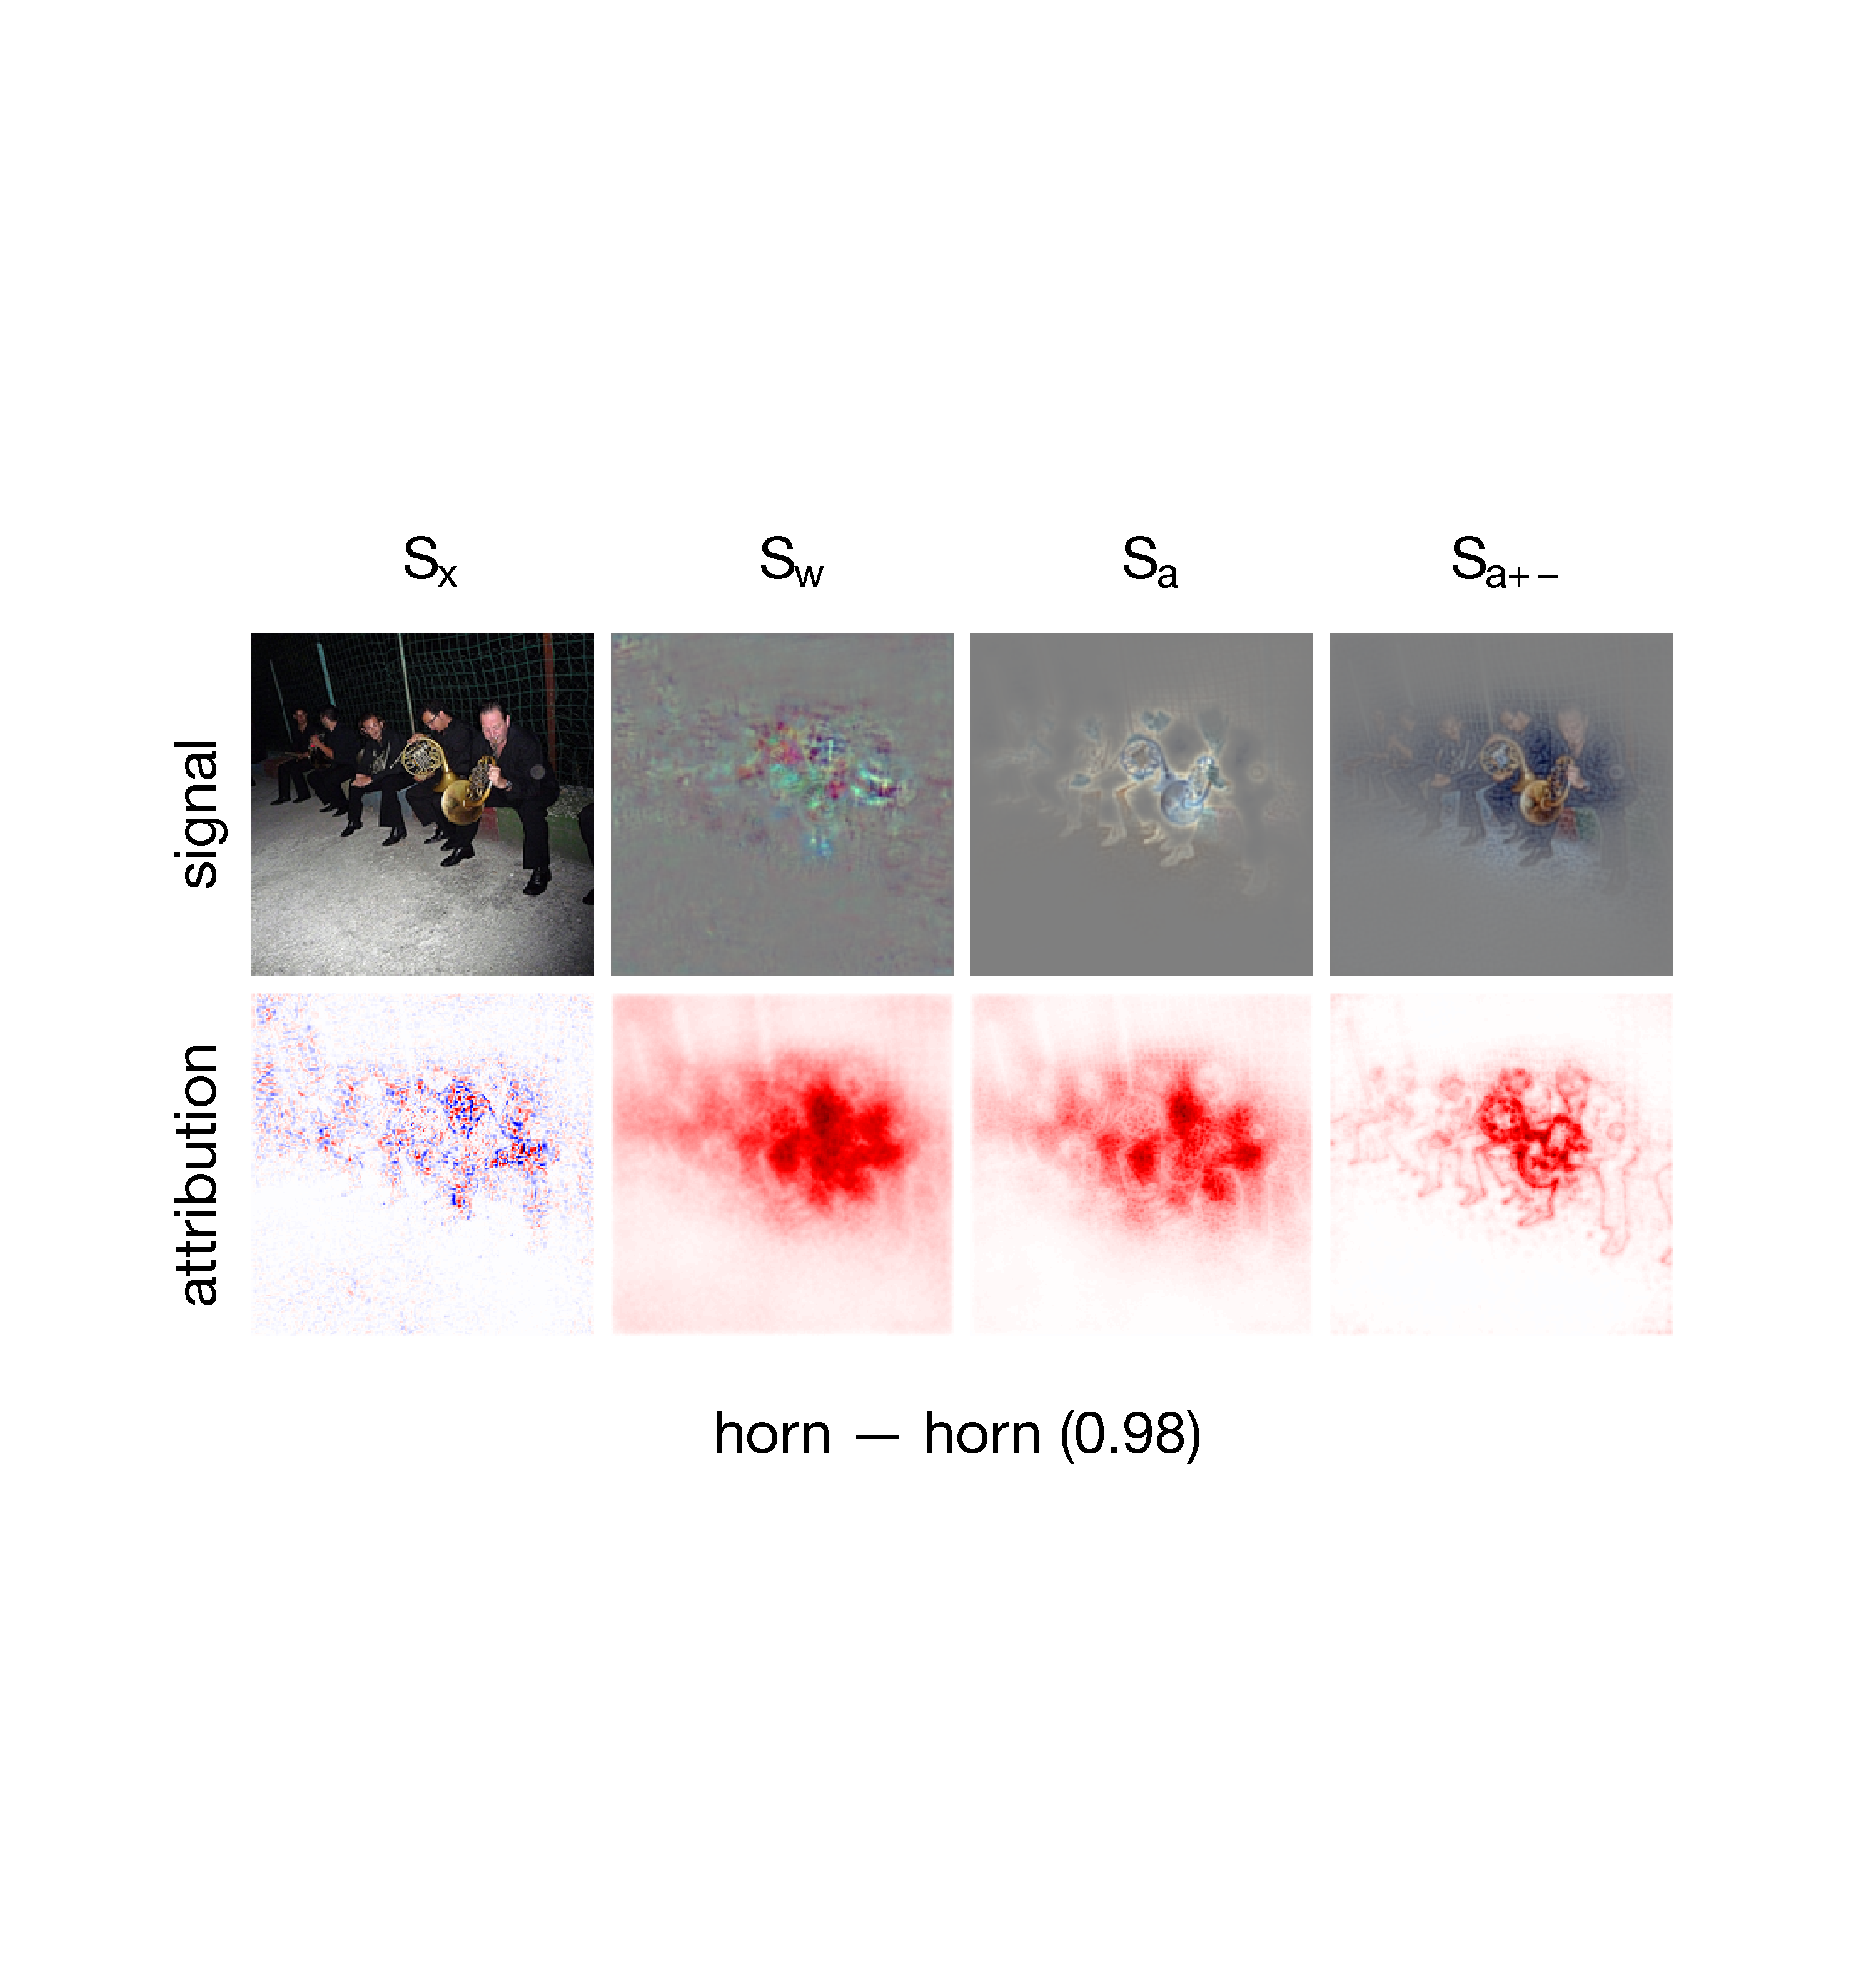
\includegraphics[width=\textwidth/2]{kindermans-signal-estimators-visually}
    \caption[Visual example for the three signal estimators.]{Visual example for the three signal estimators. \(S_x\) is the identity estimator with \(S_x(x)=x\). Figure adopted from~\cite{Kindermans.2018}}\label{fig:kindermans-signal-estimator-visually}
\end{figure}
% \subsection{CAM and GradCAM}
\blindtext[1]

% \subsection{LIFT}
\blindtext[3]
% \subsection{ProtoDash}
\blindtext[1]
% \subsection{SHAP}
\blindtext[3]
